%%%%%%%%%%%%%%%%%%%%%%%%%%%%%%%%%%%%%%%%%%%%%%%%%%%%%%%%%%%%%%%%%%%%%%%%
% Preamble
%%%%%%%%%%%%%%%%%%%%%%%%%%%%%%%%%%%%%%%%%%%%%%%%%%%%%%%%%%%%%%%%%%%%%%%%
\documentclass[11pt]{article}
%
% Packages and other includes
% Pagination
\usepackage[letterpaper, margin=1in]{geometry}
\usepackage{emptypage}
%
% Fonts
\usepackage[T1]{fontenc} % best for Western European languages
\usepackage{lmodern} % Latin Modern instead of CM
\usepackage{textcomp} % required to get special symbols
%
% Math
\usepackage{amsmath, amssymb}
\usepackage{braket}
%
% Graphics, floats, tables
\usepackage{graphicx, color, float, array}
%
% Hyperlinks
\usepackage{hyperref}
%
%
% Definitions and settings
% Paragraph indent and spacing
\setlength{\parskip}{0.4\baselineskip}
\setlength{\parindent}{0in}
%
%
% Title, authors, date
\title{\textbf{Worksheet 4}}
\date{\vspace{-2em}January 26, 2022}
%
%
%%%%%%%%%%%%%%%%%%%%%%%%%%%%%%%%%%%%%%%%%%%%%%%%%%%%%%%%%%%%%%%%%%%%%%%%
% Main document
%%%%%%%%%%%%%%%%%%%%%%%%%%%%%%%%%%%%%%%%%%%%%%%%%%%%%%%%%%%%%%%%%%%%%%%%
%

\begin{document}

\maketitle

Weekly homework assignments are posted approximately one week prior to the
due date. Collaborations are encouraged and students must report all collaborators
in writing on each assignment. All external sources (websites, books) must be
properly cited. Additional problems are listed at the end of each assignment.
This week's assignment is due \textit{Tuesday, Feb 1st at 10:00am.}

\textbf{Hess's Law}

1. (4 pts) Calculate the reaction enthalpy for the formation of anhydrous aluminum
bromide,
\begin{quote}
2 Al(s) + 3 Br$_2$(l) $\rightarrow$ 2 AlBr$_3$(s),
\end{quote}
from the following data:
\begin{quote}
2 Al(s) + 6 HBr(aq) $\rightarrow$ 2 AlBr$_3$(aq) + 3 H$_2$(g)  $\Delta H^\circ = - 1061\text{kJ}$

HBr(g) $\rightarrow$ HBr(aq) $\Delta H^\circ = -81.15\text{kJ}$

H$_2$(g) + Br$_2$(l) $\rightarrow$ 2 HBr(g) $\Delta H^\circ = -72.80\text{kJ}$

AlBr$_3$ $\rightarrow$ AlBr$_3$(aq) $\Delta H^\circ = -368\text{kJ}$
\end{quote}

\pagebreak

2. \textbf{Born--Haber Cycle} (6 pts) Ionic solids are extremely stable and lattice energy
is an additional energy contribution to the overall stability. However, the lattice
energy cannot be measured directly. The Born--Haber cycle uses the Hess's Law and allows us
to compute the lattice energies of an ionic compound. The cycle is sketched for NaCl,
\begin{center}
  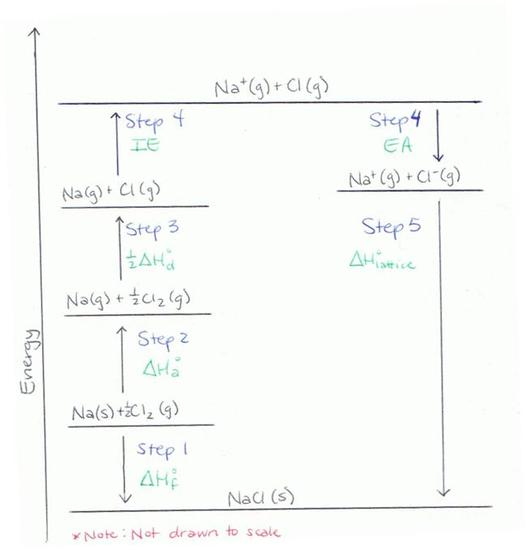
\includegraphics[scale=0.5]{born_haber_nacl.jpg}
\end{center}

This involves sublimation energy, dissociation energy, ionization energy,
and electron affinity. The sum of these processes yields the lattice energy. Repeat
this for cesium oxide (Cs$_2$O).

(a) Draw the Born--Haber cycle.

(b) Look up the enthalpy for the various processes (remember to cite) and calculate
the lattice energy of Cs$_2$O. Write all thermochemical equations for each step.

\pagebreak


\textbf{Entropy}

%Atkins 8.35

3. (4 pts) Without performing any calculations, predict whether there is an increase or
decrease in entropy for each of the following processes:

(a) Cl$_2$(g) + H$_2$O(l) $\rightarrow$ HCl(aq) + HClO(aq)

(b) SO$_2$(g) + Br$_2$(g) + 2 H$_2$O(l) $\rightarrow$ H$_2$SO$_4$(aq) + 2 HBr(aq)

(c) NaCl(s) $\rightarrow$ NaCl(aq)

(d) Cu$_3$(PO$_4$)$_2$(s) $\rightarrow$ 3 Cu$^{2+}$(aq) + 2 PO$_4^{3-}$(aq)

\vspace{1in}

4. The following is a molecular visulization of a system undergoing a spontaneous
change. Determine from the picture whether entropy increases or decreases during the
process. Account for the spontaneity of the process in terms of the entropy changes
in the system and the surroundings. The therometers show the temperature of the
system.

\begin{center}
  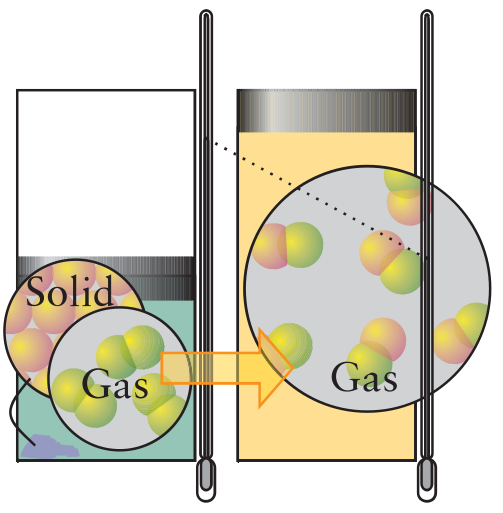
\includegraphics[scale=0.33]{entropy.png}
\end{center}


\vfill
\textbf{Optional Additional Problems:} Ch. 9 - odd problems 71 - 75, 93, 95; Ch. 18
- odd problems 27 - 41

\end{document}
